\section{Experiment and Results}
\label{sec:eval}

In this section, we explain the details about the design of experiments implemented on English and German.
Moreover, we display the results obtained by classification and word-pair difficulty ranking, including the performance on various features and comparisons between baseline models and our feature engineering model.

\subsection{Experiment Settings}
\label{sec:exper}
We choose two tasks to show the effectiveness of the multi-faceted features: For the classification task, each word will be classified into a difficulty category directly. For the ranking task, the model will tell which word is more difficult in a word pair.

We conduct the experiments on both English and German to observe the performance on various languages. 
The reason we choose these two different languages is that English and German are distant enough with quite different morphological and syntactic rules. 
%For instance, nouns in German have genders while English don't.}
There are also several experiments about text readability implemented in English and German such as Anderson's work~\shortcite{anderson1981analysing}.

%Both the word difficulty classification task and pairs ranking task are 
The word difficulty classification and word-pair difficulty ranking tasks in English is implemented on two corpora denoted as E1 and E2,
while the tasks on German is only implemented on one corpus denoted G1.

\textbf{Dataset.} 
A dataset is made up of three parts: a reliable corpus, a pronunciation dictionary and a standard leveled word list. The reliable corpus is the resource for extracting features of words, the dictionary is used to obtain phonemes of a word, and the word list is regarded as the ground truth for this task.

Table \ref{tab:src} and \ref{tab:corpus} list the source of the datasets and details of the corpora used in both English and German analysis.

It is worth emphasizing that we chose Common European Framework of Reference for Languages  (CEFR) as the ground truth, which is an authoritative standard of over 20-year work by Council of Europe~\cite{little2006common,little2011common}. 
This reference covers multiple language standards in Europe, including English, French, German and etc.
We select the relevant part for our needs -- English and German respectively.

For classification task,  the label for each word has already annotated by CEFR and can be used directly.
For ranking task, we choose the pairs of words of any two different difficulty levels according to the CEFR standard levels to make up the ranking dataset.
Each pair will be considered in both positive and negative directions which is shown as Table \ref{tab:pairs}, where $w_1$ and $w_2$ are words from different levels.

The training set and test set for both tasks are divided by a ratio of 9:1.

\begin{table}[ht]
	\begin{center}
		\scriptsize
		\begin{tabular}{|l|l|l|}
			\hline
			& \multicolumn{1}{c|}{\textbf{Resouce Description}} & \multicolumn{1}{c|}{\textbf{Resource}}                     \\ \hline
			\hline
			\multirow{4}{*}{\textbf{English}} & Corpus Resource 1   (E1)                   & \tabincell{l}{New York Times (2005-2006)}                        \\ \cline{2-3} 
			& Corpus Resource 2     (E2)                      & Gutenberg Dataset                                          \\ \cline{2-3} 
			& Pronunciation Dictionary               & CMU Pronunciation Dictionary                               \\ \cline{2-3} 
			& \tabincell{l}{Leveled Ground Truth}         & \tabincell{l}{CEFR }      \\ \hline
			\hline
			\multirow{3}{*}{\textbf{German}}  & Corpus Resource  (G1)                     & \tabincell{l}{European Parliament Proceedings \\Parallel Corpus for German} \\ \cline{2-3} 
			& Pronunciation Dictionary               & German Pronunciation Dictionary                            \\ \cline{2-3} 
			&  \tabincell{l}{Leveled Ground Truth}         & BerLiner Platz Levels  (Based on CEFR)                                    \\ \hline
		\end{tabular}
	\end{center}
\vspace{-0.25cm}
	\caption{\label{tab:src} Details of Dataset.}
\end{table}
\vspace{-0.5cm}
\begin{table}[th]
	\begin{center}
		\scriptsize
		\begin{tabular}{|c|c|c||c|}
			\hline
			\textbf{} & \multicolumn{2}{c||}{\textbf{English}} & \textbf{German} \\ \hline
			& \tabincell{c}{New York Times\\(2005-2006) (E1)}       & \tabincell{c}{Gutenberg \\ (E2)}   & \tabincell{c}{Parallel Corpus for De. \\(G1)} \\ \hline
			\tabincell{c}{Words}   & 91,082,168          & 157,196,249   & 28,423,344               \\ \hline
%			\tabincell{c}{Articles} & 177,057   & 3,037          & -               \\ \hline
			Size        & 617.06MB  & 1.13GB         & 440 MB          \\ \hline
		\end{tabular}
	\end{center}
\vspace{-0.25cm}
	\caption{\label{tab:corpus} Number of words and data size of the corpora.}
\end{table}
\vspace{-0.5cm}
\begin{table}[ht]
	\scriptsize
	\begin{center}
		\begin{tabular}{|c|c|c|c|}
			\hline
			& \textbf{Word pair} & \textbf{Description} & \textbf{Label} \\ \hline
			1 & ($w_1, w_2$) & $w_1$ is more difficulty than $w_2$. & 1 \\ \hline
			2 & ($w_2, w_1$) & $w_2$ is easier than $w_1$. & 0 \\ \hline
		\end{tabular}
	\end{center}
	\vspace{-0.25cm}
	\caption{\label{tab:pairs} Word pairs constructed for difficulty ranking task.}
\end{table}

For English, we choose The New York Times Annotated Corpus~\cite{Evan2008newyork} and Gutenberg Dataset~\cite{lahiri:2014:SRW} as the corpora to generate the features of words.
We select the New York Times articles from 2005 to 2006 and all the articles in Gutenberg Dataset.
% which contains 177,057 and 3,037 articles respectively.\JQ{ambiguity: you select these number of articles? or both contains totally these number of articles but u just use part of them? }
We choose the CMU Pronunciation Dictionary (CMUdict) to extract the phoneme components of words.
The CEFR word list for English
%, an international standard to describe language ability, 
is selected 
as the ground truth for word difficulty classification and word-pair difficulty ranking. 
%This reference covers multiple language standards in Europe, including English, French, German and etc.
%We select the relevant part for our needs -- English and German respectively.
%In the prediction of English words difficulty, the English branch of CEFR is selected. \JQ{delete}
The details of the English word levels collected from CEFR are 
shown in Table \ref{tab:CEFR}.


%The German word levels are collected from BerLiner Platz books, which is corresponding to the first three levels of CEFR.
%\JQ{why there is no B2, C1 and C2 in Table 6? How did u divide the train and test set?}\\

%    \begin{table}[th]
%	
%	\centering  
%	\subtable[The Description and Word Size of CEFR Level.]{  
%	\begin{tabular}{|c|l|c|}
%		\hline
%		\textbf{Level}&\textbf{Description}& \textbf{Words} \\
%		\hline
%		A1&Breakthrough or beginner&211\\
%		\hline
%		A2&Waystage or elementary&395\\
%		\hline
%		B1&Threshold or intermediate&718\\
%		\hline
%		B2&Vantage or upper intermediate &1215\\
%		\hline
%		C1&\tabincell{l}{Effective operational \\ proficiency or advanced} &778\\ 
%		\hline
%		C2&Mastery or proficiency&911\\
%		\hline
%	\end{tabular}
%	\label{tab:CEFR}
%	}  
%	\qquad  
%	\subtable[The Corresponding CEFR Level and Word Size of BerLiner Platz Level.]{          
%	\begin{tabular}{|c|c|c|}
%		\hline
%		\textbf{Level}&\textbf{CEFR Level}& \textbf{Words} \\
%		\hline
%		G1 & A1 & 830\\
%		\hline
%		G2 &A2&741\\
%		\hline
%		G3&B1&931\\
%		\hline
%	\end{tabular}
%	\label{tab:German}
%	}  
%\caption{Description for Two Leveled Ground truth}  
%\end{table}  

\begin{table}[ht]
	\begin{center}
		\scriptsize
		\begin{tabular}{|c|l|c|c|}
			\hline
			\textbf{CEFR Level}&\textbf{Description}& \textbf{Train} & \textbf{Test}\\
			\hline
			A1&Breakthrough or beginner& 190&21\\
			\hline
			A2&Waystage or elementary& 356& 39\\
			\hline
			B1&Threshold or intermediate& 647&71\\
			\hline
			B2&Vantage or upper intermediate & 1093&122\\
			\hline
			C1&\tabincell{l}{Effective operational \\ proficiency or advanced} & 700& 78\\ 
			\hline
			C2&Mastery or proficiency& 820&91\\
			\hline
		\end{tabular}
	\end{center}
	\vspace{-0.25cm}
\caption{\label{tab:CEFR} The description and the number of words for CEFR level.}
\end{table}

\begin{table}[]
	\begin{center}
		\scriptsize
		\begin{tabular}{|c|c|c|c|}
			\hline
			\textbf{BerLiner Platz Level}&\textbf{CEFR Level}& \textbf{Train} & \textbf{Test}\\
			\hline
			G1 & A1 & 747 & 83\\
			\hline
			G2 &A2& 667 & 74\\
			\hline
			G3&B1& 838 & 93\\
			\hline
		\end{tabular}
	\end{center}
	\vspace{-0.25cm}
	\caption{\label{tab:German} The corresponding CEFR level and the number of words for BerLiner Platz Level.}
\end{table}

For German, the German part of European Parliament Proceedings Parallel Corpus~\cite{koehn2005europarl} is used to extract word features.
A German pronunciation dictionary\footnote{\url{https://github.com/f-e-l-i-x/deuPD}} modeled after CMUdict 
%\JQ{what do u mean by "modeled after CMUdict"?} 
is chosen to generate the phoneme components of words.
The ground truth is the collection of BerLiner Platz, a three-level wordlist based on CEFR standard as shown in Table \ref{tab:German}. 

\textbf{Data Preprocessing.} To extract the features of words, we tokenize the original corpora with the help of Stanford CoreNLP~\cite{manning2014stanford}.
We define our task as a single label classification or ranking problem based on the fact that only 6.54\% of phrases and words have multiple labels in CEFR dataset.
Thus, phrases and words that belong to multiple classes are removed from the reference word lists. 
The details listed in Table \ref{tab:CEFR} and \ref{tab:German} have been filtered. 
%In order to avoid the interference caused by the  phrases and the overlap of different levels of words in the reference word lists,  we manually remove these words.
%The details in Table \ref{tab:CEFR} and \ref{tab:German} is the result after filtering.\JQ{delete}

Other procedures for getting the features has been mentioned in Section \ref{sec:feature}.
The derived features are concatenated into vectors as the input for classifiers, while the subtracted vectors are the input of the difficulty ranking model.

\textbf{Model Details}
%\textbf{Feature Details and Evaluation Metrics.} 
There are totally 10 features
%which are describe in Table \ref{tab:features} 
we considered to use, and they are discussed in Section \ref{sec:feature}. As for word embedding, 
we use different algorithms to generate word embeddings and do the parameter selection by grid-search for determining the dimension and context size
of Word2Vec and GloVe.
% and finally choose the parameters with the best performance.
For BERT, we acquire word embeddings not only by pre-trained $\text{BERT}_\text{BASE}$ and $\text{BERT}_\text{LAREG}$, but also by the $\text{BERT}_\text{BASE}$  model trained with our own corpora.
%\SY{Due to the limit of space, the results of different parameters will be shown in the Appendix.}

%\textbf{Classification and Word-pair Difficulty Ranking.} 
Based on the extracted features mentioned in Section \ref{sec:feature}, we implement both the classification model and word-pair difficulty ranking model to measure the word difficulty.
We try support vector machine (SVM), logistic regression (LR) and multi-layer perceptron (MLP) and pick the model with the best results.
For both tasks, accuracy on test set and the average accuracy on 10-fold cross validation sets are used as the metrics. All of the results are the average of 10 runs.
\subsection{Feature Selection}
% and Robustness in Different Corpora
\label{sec:embedding}
Based on the extracted features, we use the multi-layer perceptron (MLP) to measure the effectiveness of each single feature and their combination effects.
We denote the combination of all the features as ALL.
Then the performance of each individual feature is measured by removing it from ALL one at a time.

\begin{table}[ht]
	\scriptsize
	\begin{center}
		\begin{tabular}{lccc}
		\hline
		&\textbf{\tabincell{c}{\tabincell{c}{E1\\NY Times}}} & \textbf{\tabincell{c}{\tabincell{c}{E2\\Gutenberg}}} & \textbf{\tabincell{c}{G1\\German}} \\ \hline
	\textbf{ALL}&     \textbf{42.94\%}       &   \textbf{41.18\%}   &\textbf{47.74\%}         \\ \hline \hline
		\textbf{ALL-Freq}     &      40.81\%    &     40.51\%&      47.12\%          \\ 
	\textbf{ALL-Length}      &    41.72\% &  40.90\%      &  43.00\%        \\ 
	\textbf{ALL-Phoneme}   &       42.32\%        &   40.14\%    &      41.98\%             \\ 
	\textbf{ALL-BiVec}    &        42.85\%  &40.77\%&       43.00\%          \\ 
		\textbf{ALL-TriVec}   &         41.28\% &   41.11\%  &46.71\%          \\ 
	\textbf{ALL-BiProb}    &          42.04\%    &       38.98\%  &      45.06\%           \\ 
		\textbf{ALL-TriProb}  &    41.46\%        &	39.61\%      &       45.88\%         \\ 
	\textbf{ALL-POS}      &      40.70\%     &      40.93\%  &       43.21\%   \\ 
	\textbf{ALL-Dependency}&     38.65\%              &  37.52\%  &      46.71\%~            \\ 
		\textbf{ALL-Embedding} &\textbf{34.22\%}                 & \textbf{33.78\%}     & \textbf{41.36\%}        \\ \hline 
	\end{tabular}
	\end{center}
	\vspace{-0.25cm}
\caption{\label{tab:featurecompare} Classification ablation test of accuracy with each individual feature taken away. 
	Accuracy shown is the average of ten runs. The embedding in this table is Word2Vec.}
\end{table}

Table \ref{tab:featurecompare} shows the classification results of all features and the different compounds with each individual feature taken away.
In this table, we use Word2Vec to get the word embeddings.
%\SY{Do we need to mention the other embeddings?}
%, because it has a better performance than the other two embeddings which will be shown in the Appendix.
We can find that the combination of 10 features has the best performance corresponding to ALL in the first row.
The most effective features are bolded in all columns.

From the table, we have once again confirmed that word frequency is not the determining factor for word difficult and this phenomenon is more pronounced in German.

In both English corpora, the embedding and dependency are top-two effective features.
While in German, although embedding is still the best feature, we find that the intra-word features of words have a competitive performance.

To show the correctness of the above discovery, we intuitively conduct the experiments on combination of features in different aspects, and the results are in Table \ref{tab:featureL}.

\begin{table}[th]
	\scriptsize
	\begin{center}
		\begin{tabular}{lccc}
		\hline
		\textbf{}            & \textbf{\tabincell{c}{\tabincell{c}{E1\\NY Times}}}& \textbf{\tabincell{c}{\tabincell{c}{E2\\Gutenberg}}} & \textbf{\tabincell{c}{G1\\German}} \\ \hline
		\textbf{ALL}         &      \textbf{42.94\%}       &   \textbf{41.18\%}   &\textbf{47.74\%}       \\ \hline
		\hline
		\textbf{Frequency+Length} &      34.13\%       &      29.55\%       &      36.05\%       \\ 
		\textbf{Intra-word Features} &      28.14\%       &      28.45\%       &      \textbf{44.32\%}       \\ 
		\textbf{Syntactic Features}     &      31.51\%       &      30.56\%       &      39.34\%       \\ 
		\textbf{Semantic Feature}       &      \textbf{39.40\%}       &      \textbf{36.82\%}       &      37.82\%       \\ \hline
	\end{tabular}
	\end{center}
	\vspace{-0.25cm}
\caption{\label{tab:featureL} Comparison of classification accuracy on different feature aspects on three corpora.
Each accuracy is the average of ten runs. The embedding in this table is Word2Vec.}
\end{table}
 
This experiment makes an discovery that intra-word features play a very important role in German, even though in English it doesn't seem to be as important as other features. 
One reasonable explanation is that the pronunciation of 
the German word is closely related to its difficulty which can be 
discovered in Table \ref{tab:featurecompare} and German words are usually 
longer than English ones.

Comparing E1 and E2, the relative strength of different categories of features are similar, suggesting strong robustness of the model against different environments.

According to the results in Table \ref{tab:featurecompare}, word embedding extracted by Word2Vec is the strongest feature to identify word difficulty, so we will consider the effectiveness of  other word embedding models in later contrast experiments on classification and word-pair ranking tasks.

\subsection{Baseline Models}
In this section, we introduce the design of baseline models for the contrast experiments on classification and word-pair ranking tasks.
\subsubsection{Human Baseline}
To observe the limitation of human on classifying the word difficulty levels, 5 experts with educational background in foreign languages are chosen to do the classification task and word-pair difficulty ranking task respectively.
For classification task, each person was pre-trained with several words randomly selected from the standard difficulty levels, and were asked to classify 100 words according to their learning outcomes and previous knowledge.
%In order to follow the actual distribution of word levels, the words to be labeled have the same distribution.
For difficulty ranking task, each person was given 100 pairs of words to label the difficulty relation of each pair. 
The words to classify and the word pairs are randomly sampled from the word list with the same distribution.
%Then we calculate the inter-judge agreement using Cohen's Kappa measurement. 



\subsubsection{Random Baseline (Random)}
In classification task, we follow the original distribution of word levels and randomly assign a level for each word and calculate the average accuracy of 10 runs.
In difficulty ranking task, each word will be randomly assigned with a word in difficulty level to make up a word pair.
Then the accuracy will be calculated as the average of 10 runs.

\subsubsection{Frequency-Only Baseline (FO)}
%Frequency is a means of estimating the word difficulty. 
%As mentioned before, word difficulty has negative correlation with its frequency.
Frequency is a considerable feature on estimating the word difficulty.
%Some research discussed the correlation between word frequency and word difficulty, finding they are highly correlated~\cite{breland1996word}.
%There also exist some websites estimating the word difficulty based on word frequency\footnote{\url{https://www.twinword.com/api/language-scoring.php}}.

To construct the frequency-only baseline model, 
we calculate the word frequencies 
%of an open frequency dataset and a single corpus used in our experiment.
%\textbf{Frequency-only model based on the open dataset (FOMO)} calculates the English words' frequencies from SUBTLEX-UK list~\cite{van2014subtlex} and the  German words' frequencies from SUBTLEX-DE list~\cite{Bryant2011}.
%\textbf{Frequency-only model based on single corpus (FOMS)} calculates word frequencies 
based on E1, E2 and G1 respectively mentioned in Section \ref{sec:exper}.
The approach to construct the dataset for both classification and ranking tasks are the same as previous. 

%The open frequency list here means the SUBTLEX-UK list~\cite{van2014subtlex} for English or SUBTLEX-DE list~\cite{Bryant2011} for German.
%The words of SUBTLEX lists are both collected from subtitles of television programs, ordered by their frequencies.
%The single corpus used in our experiment is E1, E2 or G1 mentioned in Section \ref{sec:exper}.

\subsubsection{Frequency-Clustering Baseline (FC)}
Xiaobin Chen \shortcite{chen2016characterizing} implemented text readability classification  by calculating mean frequencies of words from vocabulary bands and clusters respectively.
In this paper, we apply the clustering method to divide the vocabulary frequency bands.
%Intuitively, the distance between two words is the difference between their frequencies, so k-means is used for cluster analysis.
Intuitively, the distance between each two words can be regarded as the difference on their frequencies. We use K-means to do the clustering.

%As expected, the results of the cluster are consistent with the word frequencies distribution.
%The results of the clustering are consistent with the frequency distribution of words.
%The clustering results on The New York Times (E1) are shown as Figure \ref{fig:cluster}.
%It's clear that the frequencies bands can be  obviously divided by clustering.
Similarly, this baseline is also implemented on different corpora and different tasks.
%\SY{reviewer 2: There is no obvious clustering here.}

%\begin{figure}[th]
%	\centering
%	%	\epsfig{file=pic/bitri.eps, width=0.9\columnwidth}
%	\includegraphics[width=1\linewidth]{pic/cluster.eps} 
%	\caption{Frequencies bands divided by clustering of the New York Times. The horizontal axis is the ranking of words ordered by difficulty, and the vertical axis is the log value of frequency.}
%	\label{fig:cluster}
%\end{figure}

%\textbf{FC Model based on the open frequency datasets (FCMO)} is implemented on English and German SUBTLEX lists.

%\textbf{FC Model based on the single corpus (FCMS)} is implemented on E1, E2 and G1 respectively.

%However, it can only achieve the accuracy of 8.91\% of in English and the accuracy of 30.14\% in German by predicting the word difficulty level by dividing the frequency of words into words.
%Once again proved that the difficulty of some words is not estimated completely by its frequency.
\subsubsection{Multi-Features Baseline (MF)}
%Several related studies in the fields of education and linguistics have mentioned that the compound of word frequency, length, the number of syllables in a word and the number of consonant clusters in a word~\cite{koirala2015word} and the compound of word frequency and POS tag~\cite{hiebert2019analysis} can be the features to measure word difficulty.
Several related studies in the field of education and linguistics combine features to do their tasks. 
The combination of frequency, length, syllables and phonemes and the number of consonant clusters is used in Koirala and Culligan's work~\shortcite{koirala2015word,culligan2015comparison}. 
Hiebert et al.~\shortcite{hiebert2019analysis} used word frequency and POS tags together to measure word difficulty.

Following these studies, we conduct the \textbf{FLSCP} (Frequency+Length+\#Syllables+\#Consonant+\#Phonemes) baseline model and \textbf{FPOS} (Frequency + POS) baseline model.
Since these studies are only theoretical research and lack of automatic classification experiments, we use MLP to do the classification and ranking tasks based on these compound features.

\subsection{Results and Discussions}
\label{sec:res}
In this part, we discuss the results of our feature engineering method and other baseline models.
%The experiment is conducted on E1, E2, E1+E2 and G1.
According to the result of the multi-class classification and difficulty ranking tasks shown in Table \ref{tab:resultsEnglish} and Table \ref{tab:resultsGerman}, we can draw the conclusion as follows.
\begin{table*}[ht]
	\scriptsize
	\begin{center}
		\begin{tabular}{lcccccccccccc}
			\hline
			& \multicolumn{4}{c}{\textbf{\begin{tabular}[c]{@{}c@{}}NY Times (E1)\end{tabular}}} & \multicolumn{4}{c}{\textbf{\begin{tabular}[c]{@{}c@{}} Gutenberg (E2)\end{tabular}}} & \multicolumn{4}{c}{\textbf{E1+E1}} \\ \hline
			& \multicolumn{2}{c}{\textbf{Classification}} & \multicolumn{2}{c}{\textbf{Ranking}} & \multicolumn{2}{c}{\textbf{Classification}} & \multicolumn{2}{c}{\textbf{Ranking}} & \multicolumn{2}{c}{\textbf{Classification}} & \multicolumn{2}{c}{\textbf{Ranking}} \\ \hline
			& \multicolumn{1}{c}{\textbf{Test}} & \multicolumn{1}{c}{\textbf{\textbf{CV}}} & \multicolumn{1}{c}{\textbf{Test}} & \multicolumn{1}{c}{\textbf{CV}} & \multicolumn{1}{c}{\textbf{Test}} & \multicolumn{1}{c}{\textbf{\textbf{\textbf{CV}}}} & \multicolumn{1}{c}{\textbf{Test}} & \multicolumn{1}{c}{\textbf{CV}} & \multicolumn{1}{c}{\textbf{Test}} & \multicolumn{1}{c}{\textbf{CV}} & \multicolumn{1}{c}{\textbf{Test}} & \multicolumn{1}{c}{\textbf{CV}} \\ \hline
			\textbf{Random}&20.57\%&20.57\%&49.85\%&49.85\%&20.57\%&20.57\%&49.85\%&49.85\%&20.57\%&20.57\%&49.85\%&49.85\%\\
			\textbf{FO}&34.20\%&33.55\%&66.10\%&64.23\%&27.94\%&29.26\%&55.13\%&57.56\%&26.91\%&28.23\%&51.92\%&53.22\%\\
			\textbf{FC}&8.23\%&8.23\%&67.50\%&67.50\%&17.53\%&17.53\%&30.36\%&30.36\%&22.41\%&22.41\%&55.00\%&55.00\%\\
			\textbf{FPOS}&33.18\%&33.47\%&52.06\%&64.14\%&29.14\%&29.14\%&52.55\%&56.93\%&28.19\%&29.28\%&54.87\%&57.41\%\\
			\textbf{FLSCP}&33.78\%&34.45\%&68.49\%&66.22\%&28.70\%&29.13\%&62.06\%&59.69\%&26.56\%&28.38\%&60.56\%&58.87\%\\\hline\hline
			%			[Fix+Word2Vec]+SVM&40.84\%&39.59\%&75.59\%&78.77\%&41.07\%&36.36\%&73.63\%&74.31\%&43.85\%&39.32\%&70.89\%&65.74\%\\
			\textbf{Fix+Word2Vec}&\textbf{42.94\%}&\textbf{37.62\%}&\textbf{74.91\%}&\textbf{72.13\%}&41.18\%&34.45\%&\textbf{74.88\%}&68.68\%&42.83\%&36.65\%&\textbf{76.29\%}&\textbf{72.76\%}\\
			%			[Fix+GloVe]+SVM&38.75\%&36.56\%&68.54\%&65.43\%&37.12\%&36.25\%&64.88\%&62.05\%&38.98\%&36\%&67.62\%&63.48\%\\
			%			[Fix+BERT]+SVM&41.76\%&39.52\%&74.15\%&77.95\%&42.46\%&40.52\%&73.5\%&78.29\%&43.85\%&40.83\%&71.93\%&79.46\%\\
			\textbf{Fix+BERT}&42.11\%&36.93\%&68.55\%&67.58\%&\textbf{41.76\%}&\textbf{35.78\%}&64.19\%&\textbf{69.12\%}&\textbf{43.23\%}&\textbf{38.92\%}&65.48\%&70.26\%\\
			\textbf{Fix+GloVe}&36.80\%&34.97\%&67.01\%&67.35\%&38.77\%&34.86\%&62.70\%&68.22\%&38.68\%&35.15\%&66.29\%&69.72\%\\\hline\hline
			\textbf{Human baseline}&49.28\%&-&88.89\%&-&49.28\%&-&88.89\%&-&49.28\%&-&88.89\%&-\\\hline
		\end{tabular}
	\end{center}
\vspace{-0.25cm}
	\caption{\label{tab:resultsEnglish} 
		The classification and ranking results 
		%		 of different baseline models and our feature engineering methods by averaging ten runs 
		for English corpora and their combination.
		The accuracy for baseline models and our feature engineering models is the average of ten runs.
		\textbf{Test} means the accuracy on test set and \textbf{CV} means the accuracy on cross validation.
		\textbf{Fix} is the compound features mentioned in this paper except word embedding.}
\end{table*}

\begin{table}[ht]
	\scriptsize
	\begin{center}
		\begin{tabular}{lcccc}
			\hline
			& \multicolumn{4}{c}{\textbf{\begin{tabular}[c]{@{}c@{}}Parallel Corpus for German (G1)\end{tabular}}} \\ \hline
			& \multicolumn{2}{c}{\textbf{Classification}} & \multicolumn{2}{c}{\textbf{Ranking}} \\ \hline
			& \multicolumn{1}{c}{\textbf{Test}} & \multicolumn{1}{c}{\textbf{CV}} & \multicolumn{1}{c}{\textbf{Test}} & \multicolumn{1}{c}{\textbf{CV}} \\ \hline
			\textbf{Random}&33.61\%&33.61\%&47.14\%&47.14\%\\
			\textbf{FO}&36.83\%&36.87\%&53.42\%&48.49\%\\
			\textbf{FC}&34.93\%&34.93\%&49.24\%&49.24\%\\
			\textbf{FPOS}&37.69\%&36.77\%&50.88\%&48.44\%\\
			\textbf{FLSCP}&39.22\%&37.46\%&52.07\%&53.67\%\\\hline\hline
			%			[Fix+Word2Vec]+SVM&42.39\%&42.46\%&70.47\%&64.23\%\\
			\textbf{Fix+Word2Vec}&\textbf{47.74\%}&\textbf{42.5\%}&\textbf{67.91\%}&\textbf{63.45\%}\\
			%			[Fix+GloVe]+SVM\%&41.98\%&42.42\%&69.07\%&65.74\%\\
			%			[Fix+BERT]+SVM\%&42.39\%&37.28\%&52.88\%&64.05\%\\
			\textbf{Fix+BERT}&46.3\%&38.98\%&54.14\%&63.32\%\\
			\textbf{Fix+GloVe}&46.91\%&41.73\%&67.51\%&69.14\%\\\hline\hline
			\textbf{Human baseline}&44.44\%&-&65.85\%&-\\\hline
		\end{tabular}
	\end{center}
\vspace{-0.25cm}
	\caption{\label{tab:resultsGerman} 
		The classification and ranking results for German corpus.
		The accuracy for baseline models and our feature engineering models is the average of ten runs.
		\textbf{Test} means the accuracy on test set and \textbf{CV} means the accuracy on cross validation.
		\textbf{Fix} is the compound features mentioned in this paper except word embedding.}
\end{table}
	
%	The explanation for this phenomenon is that FO focuses on word frequency itself and FC focuses on the frequency distribution of all words. 
%	There are more words in Gutenberg dataset which provides strong support to FC.
%	However a considerable part of words are older than those in New York Times, and this is the reason why it doesn't perform well on FOMS.

Comparing the results of FO, FC, FPOS and FLSCP under E1, E2 and E1+E2, 
we find that the accuracy on both tasks varies substantially
across different corpora.
%	Combined with the results in Section \ref{\textbf{sec:embedding}}, frequency is the best in the performance of the classification compared with length, POS and .
One possible explanation is that the large disparity in word frequency distribution leads to the unstable classification results among corpora. 
The P-value is less than 0.001 between the word frequency distribution of 
E1 and E2, which indicates there exists a significant difference.
%Thus, one possible explanation for the results is that the large disparity in word frequency distribution leads to the unstable classification results. 
Besides, 8\% of the words in test set is correctly classified in E1 while wrongly classified in E2 and E1+E2, which also supports the above conjecture.

Compared with the baselines, our proposed model takes more features 
into consideration, especially the syntactic and semantic features.
We find that the accuracy is similar among different English corpora,
namely, 42.94\%, 41.76\% and 43.23\% on classification task and 74.91\%, 74.88\% and 76.29\% on word-pair difficulty ranking task,
%Together with the results of Table \ref{tab:featureL} 
%where the relative effectiveness of different features are similar for
%different corpora, 
which shows that the performance of  multi-faceted features 
is relatively stable among different language environments.
Thus, our model has a strong generalization ability which can 
be used in diverse language environments.
	
Our proposed feature engineering model achieves the best results compared with previous models and it can achieve around 45\% on classification task and 75\% on ranking task.
Overall, all the compound features with various embeddings on different corpus environments have shown to be significantly better than the previous state-of-the-art methods by T-test with p$<$0.01.

The results in the rows corresponding to our feature engineering model show the different behaviors on different embeddings.
%Table \ref{tab:resultsEnglish} and Table \ref{tab:resultsGerman} display the best results of each embedding while others are shown in the Appendix.
The best results appear between Word2Vec and BERT, but there is no obvious advantages on BERT.
%trend on BERT.
When analyzing the features of different word embeddings, we will find that Word2Vec and GloVe combine all the different senses of word into one fixed vector. 
Different from the traditional word embedding algorithms, BERT model can capture the context of a word and clearly distinguish polysemy of a word in the sentence-level tasks.
However, when applying it to word level,  each word is represented with a fixed vector which mixes all the contextual information together and the advantage of BERT model has been defeated.

%From some prediction results of FO and ALL in Table \ref{tab:com}, we find our model can put some easy words into the correct level.
Considering the words that are wrongly predicted by FO while correctly predicted by Fix+Word2Vec, Table \ref{tab:com} lists some examples to show our model is more inclined to classify the easier ones correctly.
\begin{table}[th]
	\scriptsize
	\begin{center}
		\begin{tabular}{ccccc}
			\hline
			\textbf{Word} & \textbf{Frequency in E1} & \textbf{FO} & \textbf{ALL} & \textbf{True Label} \\ \hline
			weekday & 553 (9575/368939)& 6 & \textbf{2}& 2\\ 
			pin & 1595  (4824/368936)& 6 & \textbf{3}& 3\\ 
			birthday & 3507  (2728/368936)& 4 & \textbf{1}&  1\\ 
			coffee & 5325  (2001/368939)& 4 & \textbf{1}& 1\\ 
			\hline
		\end{tabular}
	\vspace{-0.25cm}
	\end{center}
	\caption{\label{tab:com} Prediction results of FO and Fix+Word2Vec.}
\end{table}
 As for the words that are wrongly predicted by both FO and Fix+Word2Vec, Figure \ref{fig:distance} shows the distribution of their prediction labels and the ground truth.
\begin{figure}[th]
	\centering
	%	\epsfig{file=pic/bitri.eps, width=0.9\columnwidth}
	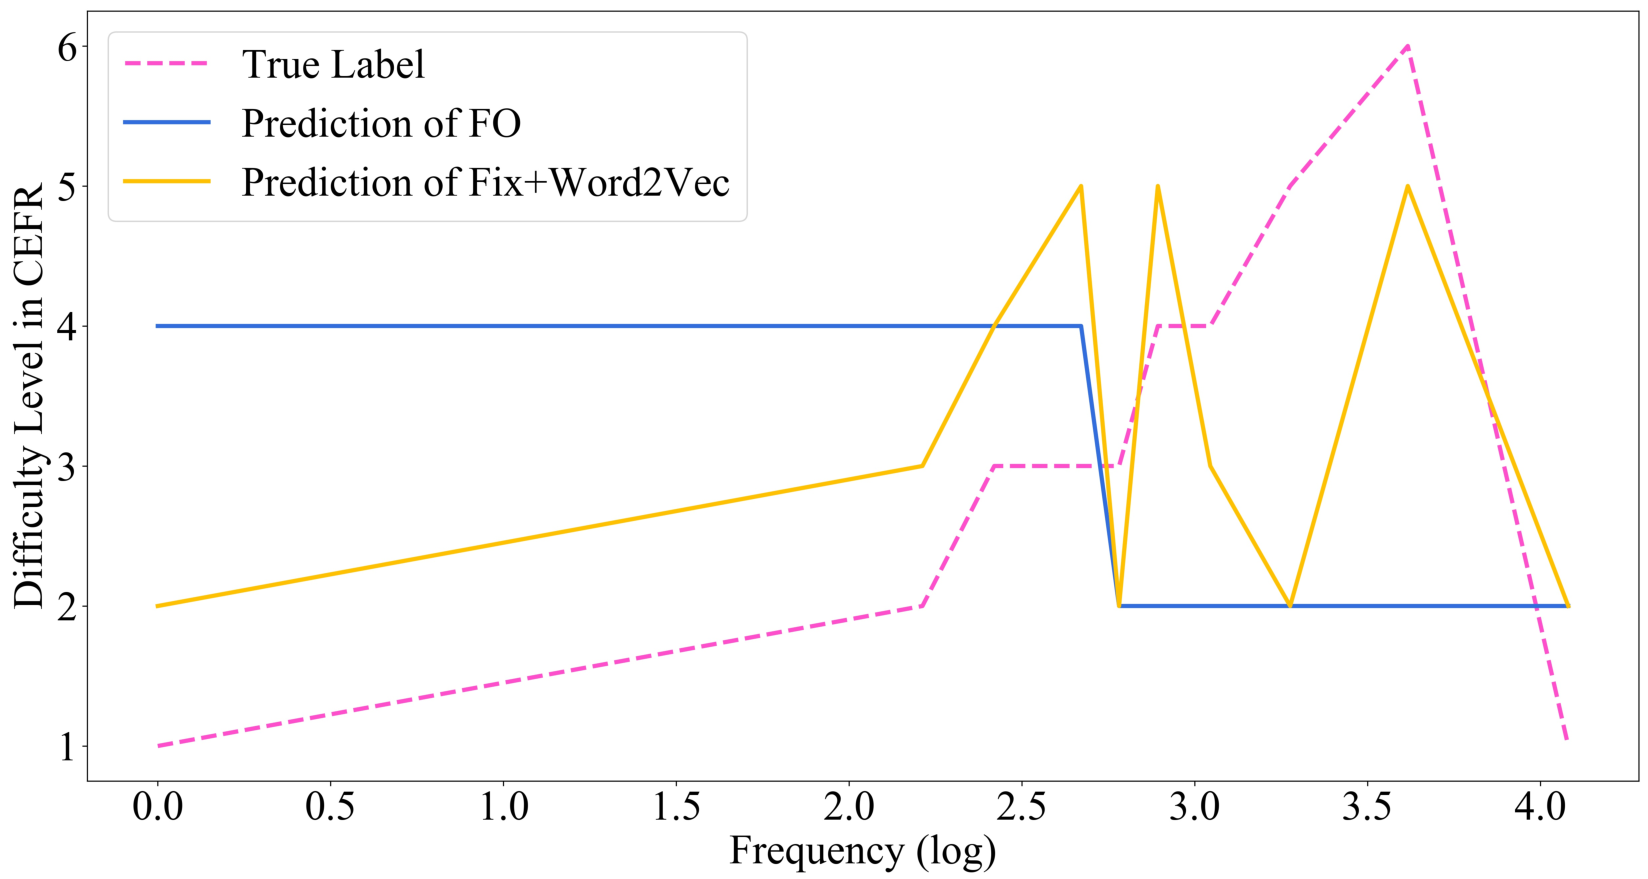
\includegraphics[width=1\linewidth]{pic/distance.pdf} 
	\vspace{-0.25cm}
	\caption{The relation between log frequency and CEFR levels.
					Lines show the distance between ground truth and wrongly predictions by FO and Fix+Word2Vec.}
	\label{fig:distance}
\end{figure}
The above results show the prediction of our multi-faceted model (Fix+Word2Vec) is more closer to the ground truth.
The correlation coefficients in Table \ref{tab:coefficients} also indicates our predictions have a certain correlation with the ground truth compared with baseline model FO.
\begin{table}[th]
	\centering
	\scriptsize
	\begin{tabular}{|c|c|c|}
		\hline
		& \textbf{Pearson} & \textbf{Spearman} \\ \hline
		\textbf{Ground Truth\&FO} & -0.057 & -0.092 \\ \hline
		\textbf{Ground Truth\&Fix+Word2Vec} & 0.305 & 0.300 \\ \hline
	\end{tabular}
	\vspace{-0.25cm}
	\caption{\label{tab:coefficients} Correlation coefficient table.}
\end{table}

The average accuracy of human classification evaluation is 49.28\% for English and 44.44\% for German.
As for difficulty ranking task, the average accuracy of human evaluation is 88.89\% for English and 65.85\% for German.
%For English, the accuracy of human labeling is 49.28\% and for German, there is an accuracy of 44.44\%.
%That is to say, human can get the correct difficulty level of words with a chance of over 45\%. As a result, our work is meaningful because it proves that people can't get a high accuracy by understanding the difficulty level of words in a short time.7
That is to say, it is a truly difficult task that even human can not achieve high accuracy given limited training. In this way, our model 
which achieves an accuracy around 45\% on classification task and 75\% on ranking task for both languages is considered very strong.
Specifically, in English, the accuracy on classification and ranking tasks is close to human behavior.
In German, the performance of our multi-faceted features is better than human.
%This result indicates that figuring out the difficulty levels manually with a short-time training is a truly difficult task. 
%In English, the classification results of multi-faceted are very close to human accuracy. 
That is to say, our work is once again shown to be meaningful and there is still room for improvement.


